\section{Пропорции в круге}

\paragraph{}\label{1938/199}
Некоторые пропорциональные линии в круге мы указали ранее (§~\ref{1938/189});
теперь укажем ещё другие.

\smallskip
\mbox{\so{Теорема}.}
\textbf{\emph{Если через точку}} ($M$, рис.~\ref{1938/ris-209}), \textbf{\emph{взятую внутри круга, проведены какая-нибудь хорда}} ($AB$) \textbf{\emph{и диаметр}} ($CD$), \textbf{\emph{то произведение отрезков хорды}} ($AM\cdot  MB$) \textbf{\emph{равно произведению отрезков диаметра}} ($MD\cdot  MC$).

Проведя две вспомогательные хорды $AC$ и $BD$, мы получим два треугольника $AMC$ и $DMB$ (покрытые на рисунке штрихами), которые подобны, так как у них углы $A$ и $D$ равны как вписанные, опирающиеся на одну и ту же дугу $BC$, и углы $C$ и $B$ равны как вписанные, опирающиеся на одну и ту же дугу $AD$.

\begin{wrapfigure}{r}{45mm}
\vskip-0mm
\centering
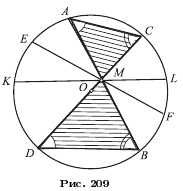
\includegraphics{mppics/ris-209}
\caption{}\label{1938/ris-209}
\end{wrapfigure}

Из подобия треугольников выводим:
\[\frac{AM}{MD}=\frac{MC}{MB}.\]
откуда
\[AM\cdot  MB=MD\cdot  MC.\]

\paragraph{}\label{1938/200}
\mbox{\so{Следствие}.}
\emph{Если через точку \emph{($M$, рис.~\ref{1938/ris-209}),} взятую внутри круга, проведено сколько угодно хорд ($AB$, $EF$, $KL,\dots$), то произведение отрезков каждой хорды есть число постоянное для всех хорд,} так как для каждой хорды это произведение равно произведению отрезков диаметра $CD$, проходящего через взятую точку $M$.

\begin{wrapfigure}{r}{50mm}
\centering
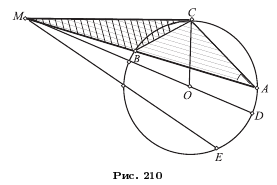
\includegraphics{mppics/ris-210}
\caption{}\label{1938/ris-210}
\end{wrapfigure}

\paragraph{}\label{1938/201}
\mbox{\so{Теорема}.}
\textbf{\emph{Если из точки}} ($M$, рис.~\ref{1938/ris-210}), \textbf{\emph{взятой вне круга, проведены к нему какая-нибудь секущая}} ($MA$) \textbf{\emph{и касательная}} ($MC$), \textbf{\emph{то произведение секущей на её внешнюю часть равно квадрату касательной}} (предполагается, что секущая ограничена второй точкой пересечения, а касательная — точкой касания).

Проведём вспомогательные хорды $AC$ и $BC$;
тогда получим два треугольника $MCA$ и $MBC$ (покрытые на чертеже штрихами), которые подобны, потому что у них угол $M$ общий и углы $MCB$ и $CAB$ равны, так как каждый из них измеряется половиной дуги $BC$.


Возьмём в $\triangle MAC$ стороны $MA$ и $MC$;
соответственными сторонами в $\triangle MBC$ будут $MC$ и $MB$;
поэтому
\[\frac{MA}{MC} = \frac{MC}{MD},\]
откуда
\[MA\cdot MB=MC^2.\]

\paragraph{}\label{1938/202}
\mbox{\so{Следствие}.}
\emph{Если из точки \emph{($M$, рис.~\ref{1938/ris-210}),} взятой вне круга, проведены к нему сколько угодно секущих ($MA$, $MD$, $ME,\dots$), то произведение каждой секущей на её внешнюю часть есть число постоянное для всех секущих, так как для каждой секущей это произведение равно квадрату касательной ($MC^2$), проведённой из точки $M$.}

%+замечание про степень точки

Величина $d^2- R^2$, где $d$ — расстояние от точки до центра окружности, a $R$ — её радиус называется \rindex{степень точки}\textbf{степенью точки} относительно окружности.
Заметим, что степень отрицательна для точек внутри круга,
положительна вне его и обращается в ноль на самой окружности.

Используя понятие степени точки, следствия приведённые в §§ \ref{1938/200} и \ref{1938/202} можно переформулировать следующим образом:
\emph{Для любой хорды $AB$ и любой точки $M$ на ней или её продолжении, произведение
\[MA\cdot MB\]
равно абсолютной величине степени $M$ относительно окружности}.


\begin{figure}[h!]
\begin{minipage}{.48\textwidth}
\centering
\includegraphics{mppics/ris-1914-228}
\end{minipage}
\hfill
\begin{minipage}{.48\textwidth}
\centering
\includegraphics{mppics/ris-1914-229}
\end{minipage}

\medskip

\begin{minipage}{.48\textwidth}
\centering
\caption{}\label{1914/ris-228}
\end{minipage}
\hfill
\begin{minipage}{.48\textwidth}
\centering
\caption{}\label{1914/ris-229}
\end{minipage}
\vskip-4mm
\end{figure}

\paragraph{}\label{1914/250}\so{Теорема}. \textbf{\emph{Произведение двух сторон треугольника равно произведению диаметра круга, описанного около этого треугольника, на высоту его, опущенную на третью сторону.}}

Обозначив буквою $R$ радиус круга, описанного около $\triangle ABC$ (рис. \ref{1914/ris-228} и \ref{1914/ris-229}), докажем, что
\[b\cdot c=2R\cdot h_a.\]

Проведём диаметр $AD$ и соединим $D$ с $B$.
Треугольники $ABD$ и $AEC$ подобны, потому что углы $B$ и $E$ прямые и $\angle D=\angle C$, как углы вписанные, опирающиеся на одну и ту же дугу.
Из подобия выводим:
\begin{align*}
\frac{c}{h_a}&=\frac{2R}{b};
\intertext{откуда:}
b\cdot c&=2R\cdot h_a.
\end{align*}
